\label{introduction}

El objetivo de esta práctica de laboratorio era realizar un diseño e implementación de un circuito digital con un juego inspirado en el arcade clásico ``Space Invaders'', en el lenguaje de descripción de hardware VHDL.

\begin{figure}[H]
	\centering
	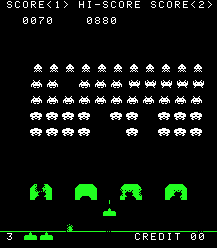
\includegraphics[width=0.4\textwidth]{SpaceInvaders-Gameplay.png}
	\caption{Pantalla del juego ``Space Invaders'' original }\label{fig:originalInvaders}
\end{figure}

Este juego, que ha sido simplificado para la consecución de este laboratorio, consiste en una nave, controlada por el jugador y localizada en la parte inferior de la pantalla, que se enfrenta a una serie de ``Invasores del espacio'', que van descendiendo por la pantalla. El jugador gana si elimina a todos los invasores, y pierde si los invasores llegan a la parte inferior de la pantalla, invadiendo la Tierra.

Para su implementación hardware se dispone de una placa entrenadora Spartar 3E Starter Board, la cual posee una FPGA Spartan 3E (modelo xc3s500E-4 FG320 ) así como distintos periféricos, como LEDs, pulsadores, interruptores, un encoder, conector VGA, etc. Para nuestra implementación hemos utilizado algunos de estos periféricos, como los LEDs, el conector VGA y 2 interruptores, así como un pin de salida, al que hemos conectado un jack de audio con un filtro paso bajo, para los sonidos y dos de los conectores de expansión de la placa, a los que hemos conectado unos mandos diseñados y construidos por nuestros compañeros del año pasado, Ruy García y Nieves Cubo, que nos los han prestado amablemente.

El desarrollo software se ha llevado a cabo usando un gestor de versiones (git) para facilitar la colaboración entre los integrantes del grupo, y se encuentra disponible de forma libre y abierta en la siguiente dirección web: 
\begin{center}
\url{https://github.com/David-Estevez/spaceinvaders} \end{center}

Se dispone también en el repositorio de una serie de etiquetas (tags) que referencian al código de cada una de las sesiones de laboratorio, de forma que es posible acceder al estado del proyecto en cada una de esas sesiones.

\newpage